
% primer permutacij pisem
\begin{figure}[H]
\centering



\tikzset{every picture/.style={line width=0.75pt}} %set default line width to 0.75pt        

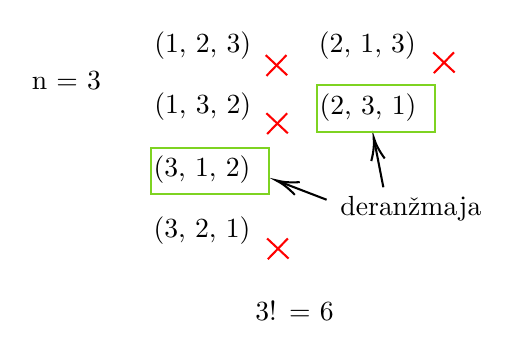
\begin{tikzpicture}[x=0.75pt,y=0.75pt,yscale=-1,xscale=1]
%uncomment if require: \path (0,300); %set diagram left start at 0, and has height of 300

%Straight Lines [id:da6274004418383881] 
\draw    (323.73,129.07) -- (319.45,107.03) ;
\draw [shift={(319.07,105.07)}, rotate = 79] [color={rgb, 255:red, 0; green, 0; blue, 0 }  ][line width=0.75]    (10.93,-3.29) .. controls (6.95,-1.4) and (3.31,-0.3) .. (0,0) .. controls (3.31,0.3) and (6.95,1.4) .. (10.93,3.29)   ;
%Straight Lines [id:da8115624533012458] 
\draw    (296.4,135.07) -- (273.93,126.45) ;
\draw [shift={(272.07,125.73)}, rotate = 20.98] [color={rgb, 255:red, 0; green, 0; blue, 0 }  ][line width=0.75]    (10.93,-3.29) .. controls (6.95,-1.4) and (3.31,-0.3) .. (0,0) .. controls (3.31,0.3) and (6.95,1.4) .. (10.93,3.29)   ;
%Shape: Rectangle [id:dp014091514879489342] 
\draw  [color={rgb, 255:red, 126; green, 211; blue, 33 }  ,draw opacity=1 ] (211.87,110) -- (268.73,110) -- (268.73,132.4) -- (211.87,132.4) -- cycle ;
%Shape: Rectangle [id:dp7623514367164748] 
\draw  [color={rgb, 255:red, 126; green, 211; blue, 33 }  ,draw opacity=1 ] (291.87,80) -- (348.73,80) -- (348.73,102.4) -- (291.87,102.4) -- cycle ;
%Straight Lines [id:da4226558851769806] 
\draw [color={rgb, 255:red, 255; green, 0; blue, 0 }  ,draw opacity=1 ]   (267.07,65.4) -- (277.4,75.07) ;
%Straight Lines [id:da934741897734465] 
\draw [color={rgb, 255:red, 255; green, 0; blue, 0 }  ,draw opacity=1 ]   (267.4,75.4) -- (277.07,65.4) ;
%Straight Lines [id:da9519310417955766] 
\draw [color={rgb, 255:red, 255; green, 0; blue, 0 }  ,draw opacity=1 ]   (347.73,64.07) -- (358.07,73.73) ;
%Straight Lines [id:da3579679185386795] 
\draw [color={rgb, 255:red, 255; green, 0; blue, 0 }  ,draw opacity=1 ]   (348.07,74.07) -- (357.73,64.07) ;
%Straight Lines [id:da23241482471605712] 
\draw [color={rgb, 255:red, 255; green, 0; blue, 0 }  ,draw opacity=1 ]   (267.4,93.4) -- (277.73,103.07) ;
%Straight Lines [id:da029077654671084252] 
\draw [color={rgb, 255:red, 255; green, 0; blue, 0 }  ,draw opacity=1 ]   (267.73,103.4) -- (277.4,93.4) ;
%Straight Lines [id:da5335697143397757] 
\draw [color={rgb, 255:red, 255; green, 0; blue, 0 }  ,draw opacity=1 ]   (267.73,153.73) -- (278.07,163.4) ;
%Straight Lines [id:da38781437837538046] 
\draw [color={rgb, 255:red, 255; green, 0; blue, 0 }  ,draw opacity=1 ]   (268.07,163.73) -- (277.73,153.73) ;

% Text Node
\draw (211.87,52.67) node [anchor=north west][inner sep=0.75pt]   [align=left] {(1, 2, 3)};
% Text Node
\draw (211.87,82) node [anchor=north west][inner sep=0.75pt]   [align=left] {(1, 3, 2)};
% Text Node
\draw (211.53,142) node [anchor=north west][inner sep=0.75pt]   [align=left] {(3, 2, 1)};
% Text Node
\draw (291.53,82.33) node [anchor=north west][inner sep=0.75pt]   [align=left] {(2, 3, 1)};
% Text Node
\draw (211.53,112.33) node [anchor=north west][inner sep=0.75pt]   [align=left] {(3, 1, 2)};
% Text Node
\draw (291.2,52.67) node [anchor=north west][inner sep=0.75pt]   [align=left] {(2, 1, 3)};
% Text Node
\draw (301.53,131.67) node [anchor=north west][inner sep=0.75pt]   [align=left] {deranžmaja};
% Text Node
\draw (152.87,72) node [anchor=north west][inner sep=0.75pt]   [align=left] {n = 3};
% Text Node
\draw (260.53,182.4) node [anchor=north west][inner sep=0.75pt]   [align=left] {3! = 6};


\end{tikzpicture}
\end{figure}